\chapter{Hardwarové komponenty} \label{chap:hw}
K provozování určitých součástí systému a měření 4 příznaků je nutné použít fyzické technické vybavení, označované také jako hardware. Tato kapitola popisuje jeho funkční celky složené z jednotlivých použitých součástí a zmiňuje využití hardwaru, které je blíže specifikováno v příslušných kapitolách (\cref{chap:dataCollection,chap:gui}).

K měření příznakových veličin (\cref{chap:features}) intenzity osvětlení a teploty vzduchu ve vnějším a vnitřním prostředí se využívá 2 desek plošných spojů (\acrshort{dps}) vlastní konstrukce osazených modulem ESP-12E od společnosti Ai-Thinker (\cref{sec:senzory}). Na jednodeskovém počítači Raspberry Pi 2B, běží následující SW součásti:
\begin{itemize}
    \item skript \file{mqttDataCollector.py}, který pomocí MQTT komunikuje s ostatními uzly a sbírá z nich data;
    \item skript \file{broker2mongo.py}, který sesbíraná data ukládá do databáze MongoDB;
    \item MQTT broker\footnote{MQTT broker je centrální uzel, který zprosdředkovává přenos zpráv od klienta, který zprávu odeslal, ke klientům, kteří se přihlásili k jejich odběru. Více v \refskl{sec:MQTT}{sekci}.} Mosquitto, ke kterému jsou připojeny všechny zdroje dat.
\end{itemize}
\label{list:rpi}
Posledním využívaným celkem je workstation označovaná jako KKY-PC, která:
\begin{itemize}
    \item Hostuje databázový server MongoDB.
    \item Hostuje webový server vlastního grafického uživatelského rozhraní (\acrshort{gui}).
    \item Provozuje vlastní REST a WebSocket backend implementovaný ve frameworku Tornado.
    \item Sloužila k trénování neuronových sítí regresorů.
\end{itemize}
Jedná se o výkonný osobní počítač s 6~jádrovým 64~bitovým procesorem Intel Core i7-7800X, 64~GiB operační paměti a grafickou kartou NVIDIA GTX 1080. Pohání ji operační systém Ubuntu 20.04.3 a po dobu vývoje běžela na Katedře kybernetiky Západočeské univerzity v Plzni.

\section{Zařízení pro měření teploty vzduchu a intenzity osvětlení} \label{sec:senzory} %Zařízení pro měření teploty a osvětlení? Senzory teploty vzduchu a intenzity osvětlení?
    Čtyři z příznaků pro regresory tvoří teplota vzduchu a intenzita osvětlení, obojí v interiéru i exteriéru. Obě veličiny byly měřeny periodicky každých 5~minut a v případě změny stavu žaluzie uživatelem pomocí již v úvodu této kapitoly zmíněných, osazených \acrshort{dps}. Jednotlivá měření se předávají po WiFi dalším součástem systému pomocí protokolu MQTT.
    
    Jedna z \acrshort{dps} je umístěna na polici v žaluzií zatemňované místnosti v domě autora tak, aby na připojené senzory nedopadalo přímé sluneční světlo. Druhá je položena na střeše tohoto domu uvnitř krabičky s průhledným okénkem tak, aby byla elektronika krytá před povětrnostními vlivy, ale na senzor intenzity osvětlení i tak dopadalo světlo. Voděodolnost krabičky zajišťuje přišroubované víko se silikonovým těsněním a silikonem utěsněné kabelové průchodky. Umístění na střeše bylo zvoleno tak, aby senzor intenzity osvětlení nebyl zastíněn dalšími nesouvisejícími předměty na střeše, jako jsou antény, jejich stožáry, komíny atp. Teplotní senzor vyvedený na kabelu o délce $0{,}75~\textrm{m}$ je umístěn za severní hranou střechy, kde je krytý před dopadajícím slunečním zářením. Fotografie skutečného umístění zařízení je na \refskl{fig:senzor}{obrázku}. Napájecí kabel je zatížen betonovou kostkou, aby se předešlo samovolnému pohybu zařízení po střeše vlivem silného větru.
    \begin{figure}
        \centering
        \includegraphics[draft=\draftfig,width=0.47\textwidth]{img/hw/IMG_20220322_182514.jpg}
        \caption[Skutečné umístění měřicího zařízení]{Skutečné umístění měřicího zařízení na střeše rodinného domu.}
        \label{fig:senzor}
    \end{figure}
    
    Hlavními součástmi těchto zařízení, které jsou podrobněji popsány dále, jsou: \acrshort{dps}, modul ESP-12E s \acrshort{mcu} ESP8266, modul se senzorem intenzity osvětlení TSL2591 a vodotěsný senzor teploty DS18B20 na kabelu. Na desce je dále přítomno 5 pasivních součástek, z toho 3 rezistory a 2 kondenzátory, a 2 tlačítka. Napájeny jsou síťovými zdroji stejnosměrného proudu o velikosti až 0{,}5~A a napětí 5~V.
    \subsection{Zapojení}
        Zapojení vychází z dokumentace součástek a jeho schéma je na \refskl{fig:schema}{obrázku}. Do paměti \acrshort{mcu} je nutné nahrát firmware, nejjednodušší možnost je využít vyvedeného rozhraní UART na pinech 15 a 16, dále k tomu slouží tlačítko \texttt{SW2}, které připojí GPIO0 na 0~V a přepne tak \acrshort{mcu} do režimu nahrávání firmwaru. Společně s napájecími piny je tedy toto rozhraní vyvedeno z desky na konektoru J1 se 4 piny. Tlačítko \texttt{SW1} slouží k propojení REST pinu (1) \acrshort{mcu} a $0~\texttt{V}$, což vyvolá jeho reset. Jinak je přes pull-up rezistor R1 připojen na napájecí napětí, aby se předešlo náhodnému resetování. Rezistor R2 pak přivádí napětí na CH\_PD pin, který tak uvede do chodu interní regulátory napětí pro procesor. Kondenzátory C1 a C2 slouží k vyhlazení napájecího napětí, omezení rušení a překlenutí odběrových špiček. Pro připojení senzoru teploty se využívá sběrnice 1-Wire, její datový vodič je připojen jednak na GPIO2, jednak přes rezistor R3 na napájecí napětí jako pull-up. Napájecí vodiče sběrnice jsou přímo spojené s napájecími vodiči \acrshort{mcu}.

        Na GPIO4 a GPIO5 jsou zapojeny po řadě datový a hodinový vodič sběrnice I$^2$C, která slouží ke komunikaci se senzorem intenzity osvětlení. Ten dále slouží jako stabilizovaný zdroj napětí pro celé zařízení, součástí modulu je totiž lineární snižující zdroj napětí o velikosti 3{,}3~V.
        \begin{figure}
            \centering
            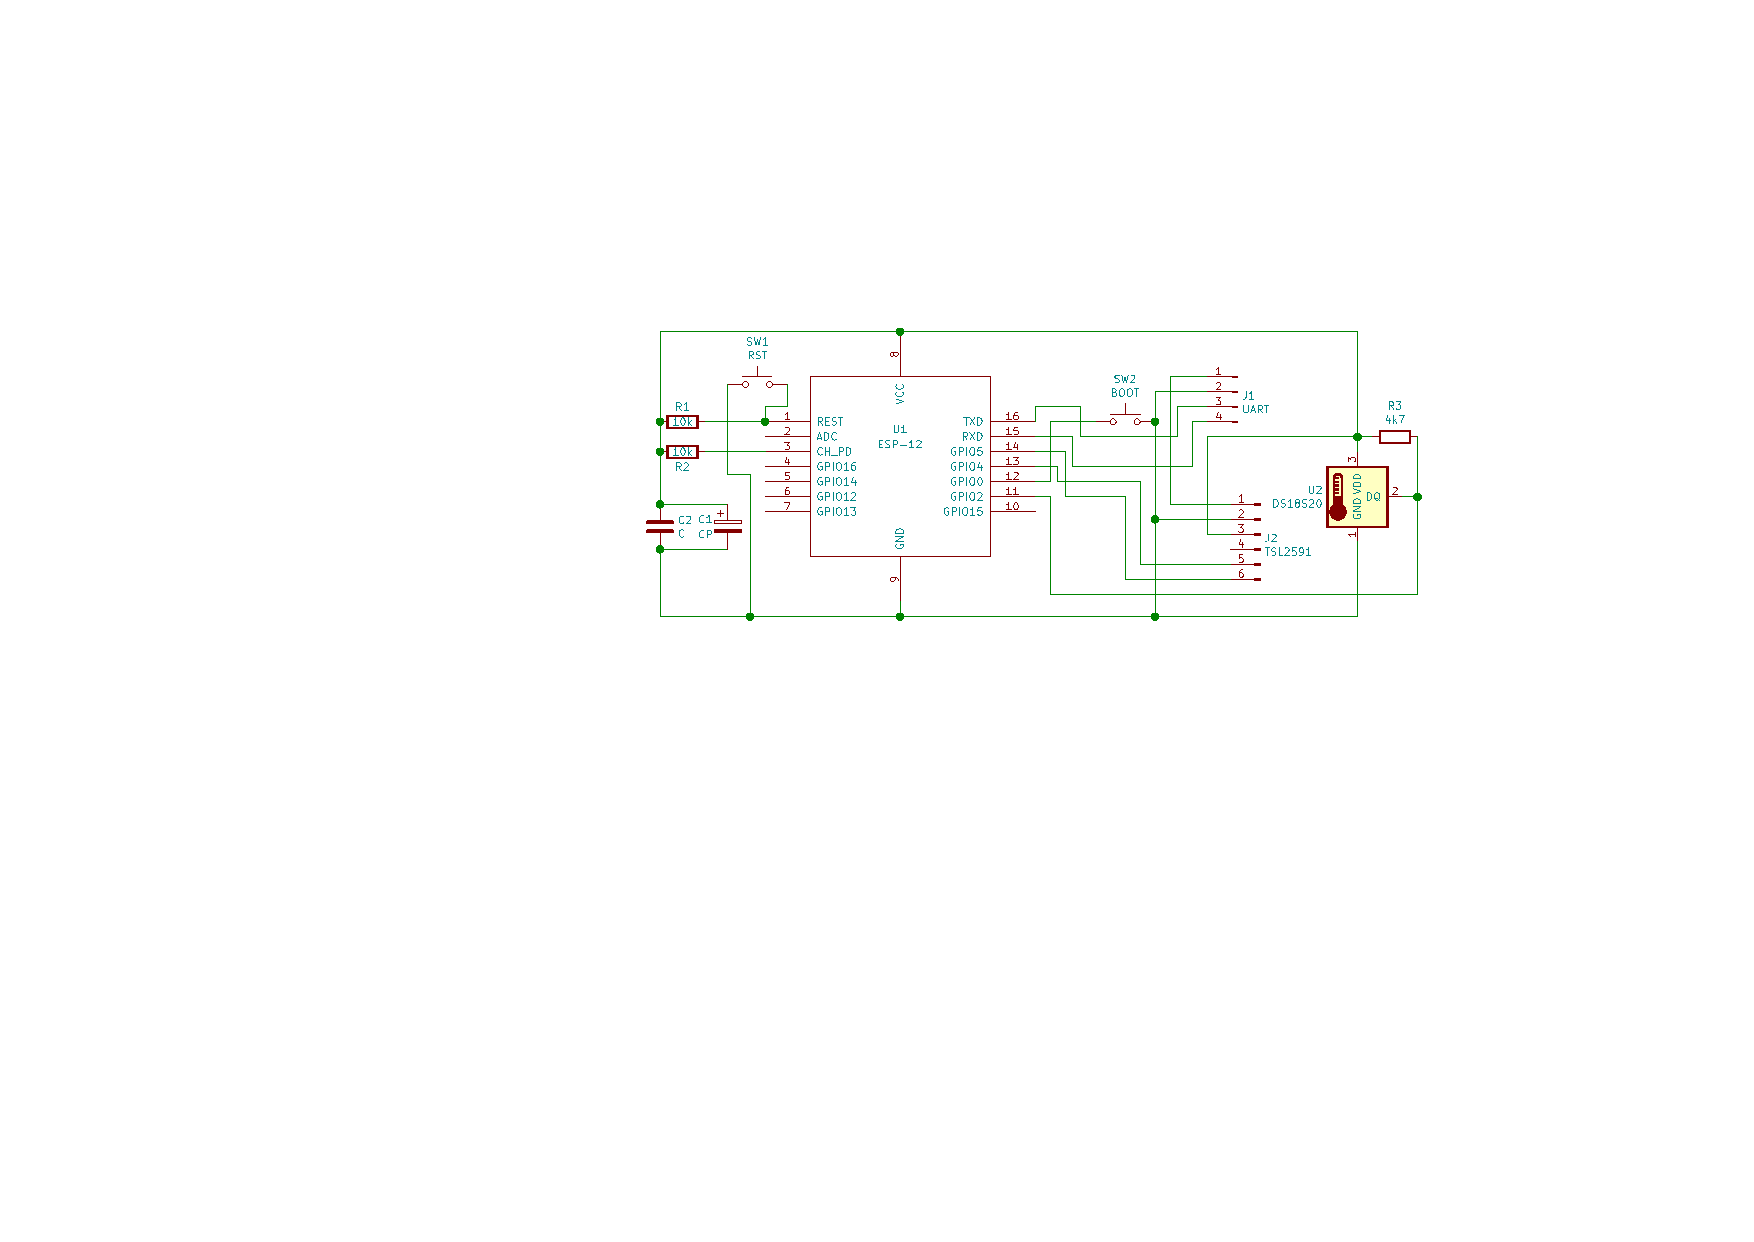
\includegraphics[draft=\draftfig,width=\textwidth,trim={10.8cm 10cm 5.5cm 5.3cm},clip]{img/hw/esp_lux_temp_sch.pdf}
            \caption[Schéma zapojení měřicích zařízení]{Schéma zapojení zařízení, která měří intenzitu osvětlení pomocí senzoru TSL2591 a teplotu vzduchu pomocí senzoru DS18B20. Hodnoty se přenáší přes WiFi.}
            \label{fig:schema}
        \end{figure}
    \subsection{\Acrlong{dps} (\acrshort{dps})}
        \acrshort{dps} elektricky propujuje ostatní komponenty těchto zařízení a byla vyrobena po domácku. V opensource programu pro návrh elektronických zařízení KiCad byl sestaven obvod a návrh \acrshort{dps} (\cref{fig:dps}), jenž byl pomocí kancelářské tiskárny překlopeně vytištěn na běžný papír v měřítku 1:1.
        
        Z jednostranně poměděného laminátu (cuprextit) byla pákovými nůžkami vystřižena deska o příslušných rozměrech dle návrhu, přebroušena brusným papírem a byla zabalena do papíru s návrhem tak, aby strana s mědí překrývala celou oblast návrhu, který byl ponechán na vnější straně. Kladivem a důlčíkem se do mědi poklepem na důlčík vyznačily budoucí díry pro jednotlivé součástky (v návrhu černá mezikruží, ze kterých mohou vést cesty) a krajní body pro osazení modulu ESP-12E (v návrhu černé obdélníky, ze kterých mohou vést cesty). Takové značky slouží jednak k orientaci při zakreslování vodivých cest, ale také při následném vrtání jako vodítko pro vrták.
        
        Po vyznačení všech děr byla deska vyňata z papíru a lihovým fixem se zakreslily pájecí body součástek (černá mezikruží a obdélníky) a cesty mezi nimi podle papírové předlohy (nejtenčí linie jsou ohraničení součástek a jejich pouzder a do desky se nezakreslují, protože nemají tvořit vodivé spojení). Pájecí body pro modul U1 (tedy ESP-12E) byly zakresleny pomocí samotného modulu použitého jako šablony zarovnané s důlčíkem vyznačenými krajními body.
        
        Přebytečná měď, která nebyla překryta barvou, se vyleptala při pokojové teplotě v roztoku chloridu železitého pro leptání plošných spojů za 25~minut a na desce tak zůstaly jen potřebné vodivé cesty. Leptání proběhlo tak, že se deska položila na hladinu roztoku nalitého do plastové leptací vaničky. Díky tomu mohly produkty chemické reakce klesat ke dnu a uvolnit prostor ještě nepoužitému roztoku. Deska byla několikrát z lázně vyjmuta a vizuálně zkontrolována, jestli barva nebyla smyta a jestli je ještě potřeba leptat dále. Když už na desce zbývaly jen části překryté barvou, tedy cesty a pájecí body, se barva očistila technickým lihem pomocí vatového polštářku a do desky se vyvrtaly otvory pro součástky. Nakonec byla deska znovu přebroušena a opatřena pájitelným ochranným lakem (v tomto případě kalafunou rozpuštěnou v lihu). Součástky byly osazeny na příslušná místa dle návrhu desky a schématu.
        \begin{figure}
            \centering
            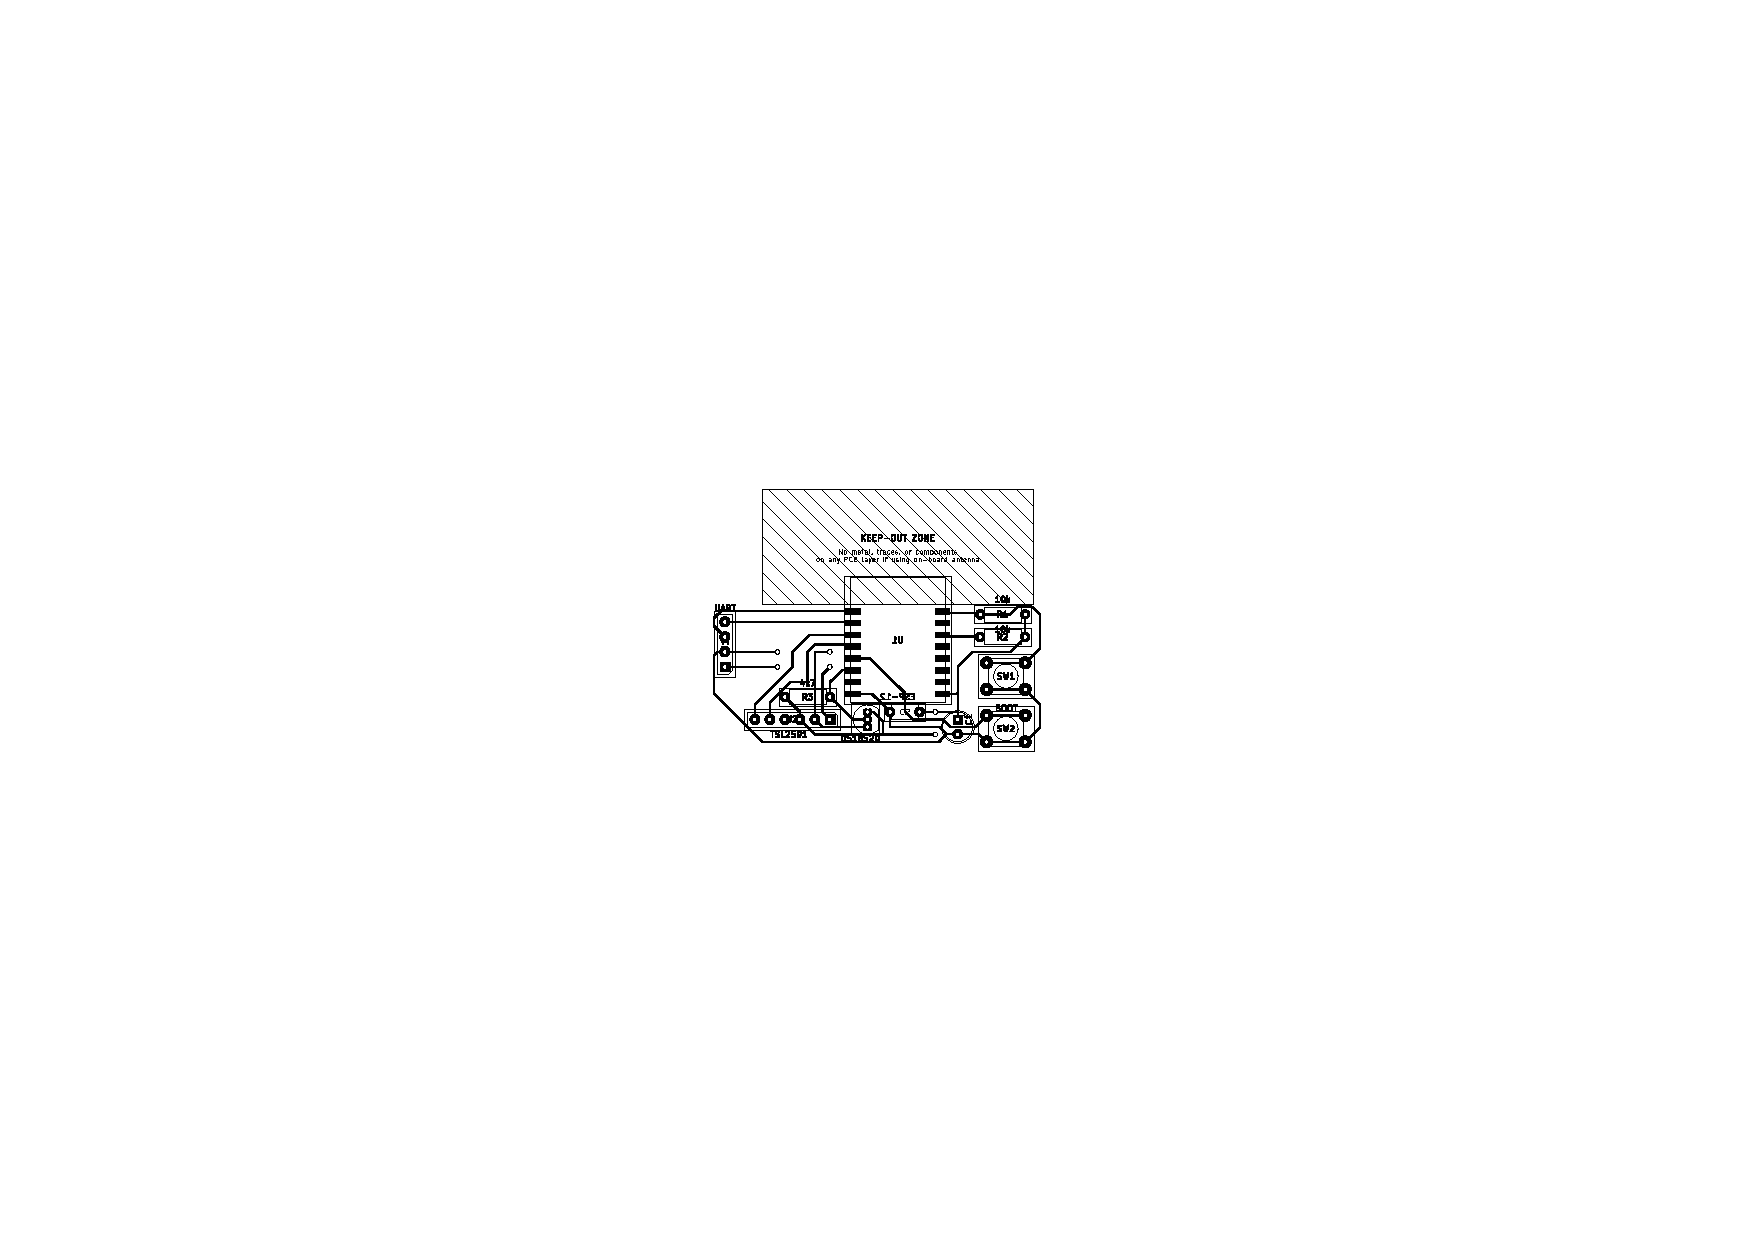
\includegraphics[draft=\draftfig,width=0.8\textwidth,trim={11.8cm 8.2cm 11.8cm 9.7cm},clip]{img/hw/esp_lux_temp_dps.pdf}
            \caption[Návrh \acrshort{dps} měřicích zařízení]{Návrh desky plošných spojů zařízení, která měří intenzitu osvětlení pomocí senzoru TSL2591 a teplotu vzduchu pomocí senzoru DS18B20. Hodnoty se přenáší přes WiFi. Šrafovaná oblast je ochranná zóna antény.}
            \label{fig:dps}
        \end{figure}
    \subsection{Modul ESP-12E s \acrshort{mcu} a WiFi}
        Modul ESP-12E vyvíjený společností Ai-thinker Team obsahuje čip ESP8266, který integruje kompletní řešení WiFi, 32~bitový procesor \emph{Tensilica L106 Diamond Series}, taktovaný na 80~MHz, s vestavěnou SRAM a 16 univerzálních vstupně-výstupních pinů. Další součástí modulu je flash paměť připojená přes rozhraní SPI, na kterou se ukládá program. \cite{ai-thinker:esp12e} V popisovaném měřicím zařízení slouží tento modul ke zpracování dat naměřených pomocí senzorů teploty a intenzity osvětlení a jejich přenosu do dalších součástí systému.
    \subsection{Teplotní senzor DS18B20}
        DS18B20 je digitální teploměr s volitelnou přesností 9~--~12~bitů, který svá měření poskytuje po sběrnici 1-Wire, k jeho provozu tedy postačuje pouze datový a zemnící vodič. Volitelně lze také připojit napájecí napětí o velikosti 3~--~5{,}5~V třetím vodičem. Na stejné sběrnici může být připojeno více teploměrů DS18B20, protože každý z nich má z výroby přidělené unikátní sériové číslo. Je dostupný v pouzdrech TO92 a SOP8 a nalezne využití ve stavebnictví při řízení vytápění, ventilace nebo klimatizace, měření teplot v budovách, v průmyslu při měření a monitorování teploty zařízení nebo procesů a jejich řízení. (\cite{dallas:ds18b20}) V měřicím zařízení poskytuje data o teplotě vzduchu.
    \subsection{Senzor intenzity osvětlení TSL2591}
        TSL2591 je digitální senzor intenzity osvětlení, který pracuje ve viditelném a infračerveném spektru. Parametry měření, kterými jsou zesílení a čas integrace, jsou volitelné a je tak možné měřit intenzitu osvětlení od 188~µlux do $88000$~lux. Měření lze číst po standardní sběrnici I$^2$C, která využívá dvou vodičů - datový vodič a vodič s hodinovým signálem. Použitý modul od firmy Adafruit s tímto integrovaným obvodem má také vlastní lineární regulátor napětí MIC5225 proudově zatížitelný až do 150~mA. (\cite{adafruit:tsl2591}) Proto byl kromě měření intenzity osvětlení interiéru i exteriéru využit také pro napájení celého zařízení z rozšířených 5~V USB síťových zdrojů (např. adaptéry pro nabíjení spotřební elektroniky).
